%\documentclass[twocolumn]{article}
%\usepackage[utf8]{inputenc}
%\documentclass[10pt,journal,onecolumn]{IEEEtran}
%\documentclass[10pt,journal,compsoc]{IEEEtran}
\documentclass[10pt, journal, letterpaper]{IEEEtran}
%\documentclass[10pt,journal,compsoc]{IEEEtran}


% NB hyperref package may need to be commented for Latex upload
\usepackage{cite}
%\ifCLASSOPTIONcompsoc
%\ifCLASSINFOpdf
% \usepackage[pdftex]{graphicx}
% declare the path(s) where your graphic files are
% \graphicspath{{../pdf/}{../jpeg/}}
% and their extensions so you won't have to specify these with
% every instance of \includegraphics
% \DeclareGraphicsExtensions{.pdf,.jpeg,.png}
%  \usepackage[nocompress]{cite}
%  \else
% normal IEEE
%  \usepackage{cite}
%  \fi

%  \ifCLASSINFOpdf

%  \else
%\fi
%important package
\usepackage{multirow} 
\usepackage{algpseudocode}
\usepackage{algorithm}
\usepackage{rotating}
\usepackage{kantlipsum} %with the next two command (commath, allowdisplaybreaks) -> allow to break the formulas along the pages
\usepackage{commath}
\allowdisplaybreaks
\usepackage{mathtools}  %with the next command adjust the vertical space between formulas
%\setlength{\jot}{5pt}
%\usepackage{ragged2e}   %if add \justify at each line, that line would be justified. This is used because the abstract of transaction style is not justified  ---- it is not compatible with twocolumn-IEEETrans
%not important
\usepackage{verbatim}
\usepackage{xr-hyper} 
\usepackage{enumitem}
\usepackage{multirow}
\usepackage[table,xcdraw]{xcolor}
\usepackage{array,arydshln}
\usepackage{graphicx,booktabs}
\usepackage{longtable}
%strikethrough not working when nested in a definition
%\usepackage[normalem]{ulem}
%\usepackage{soul}
%\usepackage{fullpage} 
%%%%%%%%%%%%%%%%%%%%%%%%%%%%%%%%%%%%%%%%%%%%%%%%%%%%%%%%%%%%%%%%%%%%%%%%%%%%%
% hyperref package may need to be commented for Latex upload
%\usepackage[pdfusetitle, pdfauthor={Michael Shell, My institution}]{hyperref}
%%%%%%%%%%%%%%%%%%%%%%%%%%%%%%%%%%%%%%%%%%%%%%%%%%%%%%%%%%%%%%%%%%%%%%%%%%%%%
\usepackage{balance}
\usepackage{flushend}
\usepackage{epstopdf}
\usepackage{wrapfig}
\usepackage{latexsym}
\usepackage{amssymb}
\usepackage{amsthm}
\usepackage{amsfonts}
\usepackage{amsmath} %[cmex10]
%\usepackage{flushend} %********************* This package has a bug: Do no include it
\usepackage{graphicx}
\usepackage{latexsym}
\usepackage{booktabs}
\usepackage[style=base]{caption}
\usepackage{subcaption} %******************* This package has conflict with sufig and subfigure
%\usepackage{subfigure}
%\usepackage{subfig}
\usepackage{breqn}
\newtheorem{thm}{Property}
\newtheorem{thm1}{Theorem}
\newtheorem{thm3}{Proposition}
\newtheorem{thm5}{Remark}
\newtheorem{thm7}{Lemma}
\algnewcommand\algorithmicinput{\textbf{INPUT:}}
\algnewcommand\INPUT{\item[\algorithmicinput]}
\algnewcommand\algorithmicoutput{\textbf{OUTPUT:}}
\algnewcommand\OUTPUT{\item[\algorithmicoutput]}
\usepackage[table]{xcolor}
%\usepackage[dvipsnames]{xcolor}
%\usepackage[cmyk]{xcolor}
%\usepackage{natbib}
\usepackage{graphicx}
\usepackage{mathtools}
\usepackage{enumitem,kantlipsum}
\usepackage{adjustbox}
% change the width and height of rows and columns in Tables
\usepackage[thinlines]{easytable}

\algdef{SE}[DOWHILE]{Do}{doWhile}{\algorithmicdo}[1]{\algorithmicwhile\ #1}
\makeatletter
\algnewcommand{\LineComment}[1]{\Statex \hskip\ALG@thistlm \texttt{#1}}
\makeatother
\newcommand{\export}{Exportation\xspace}
\newcommand{\move}{Move\xspace}
\newcommand{\ouralgorithm}{GPE\xspace} %%Green path exportation

\newlength\mylength
\setlength\mylength{\dimexpr.13\columnwidth-1\tabcolsep-0.2\arrayrulewidth\relax}
\usepackage{color}
% we need a better fix for this, see https://tex.stackexchange.com/questions/64298/error-with-xcolor-package
\colorlet{BLUE}{blue}
\usepackage{colortbl}
\definecolor{LightCyan}{RGB}{155, 227, 247}
%\captionsetup[figure]{belowskip=-8pt}
%in test

%\usepackage{nomencl}
%\makenomenclature
%% This code creates the groups
% -----------------------------------------
%\usepackage{etoolbox}
%\renewcommand\nomgroup[1]{%
%	\item[\bfseries
%	\ifstrequal{#1}{P}{Parameters}{%
%		\ifstrequal{#1}{V}{Variables}{%
%			\ifstrequal{#1}{I}{Indices}{%
%				\ifstrequal{#1}{B}{Binary~Variables}{}}}}%
%	]}

%DOUBLE QUOTATION COMMAND
\newcommand{\dq}[1]{``#1''}

% To remove all comments, comment out the definition and use the commented-out
% empty definition below
% otherwise you can comment the line \commentsontrue 
\newcommand{\commentBy}[3]{\textcolor{#1}{\textbf{#2:} #3}}
%\newcommand{\commentBy}[3]{\ignorespaces}

\newif\ifcommentson
%uncomment the line below to show comments
\commentsontrue

\newcommand{\ste}[1]{\ifcommentson \commentBy{blue}{SS}{#1} \fi}
%\newcommand{\lc}[1]{\ifcommentson \commentBy{blue}{LC}{#1} \fi}
\newcommand{\mm}[1]{\ifcommentson \commentBy{orange}{MM}{#1} \fi}

\newif\ifextended
\newif\ifshortver

%%% Show only short version in black
%%%        \shorvetrue 
%%%        %\extendedtrue 

%%% Show only extended version in black
%%%        %\shorvetrue 
%%%        \extendedtrue 

%%% Show short version in blue and extended version in purple
%%%        \shorvetrue 
%%%        \extendedtrue 

\shortvertrue
%\extendedtrue

\newcommand{\extended}[1]{\ifextended \ifshortver \textcolor{purple}{#1} \else \textcolor{black}{#1} \fi  \fi}
\newcommand{\shortver}[1]{\ifshortver \ifextended \textcolor{blue}{#1} \else \textcolor{black}{#1} \fi \fi}

%\newcommand{\optional}[1]{#1}
%\newcommand{\optional}[1]{\textcolor{Orange}{#1}}
\newcommand{\optional}[1]{\ignorespaces}


\newif\ifrevisionactive
\newif\ifshowdeleted
\revisionactivetrue
%\showdeletedtrue

\newcommand{\revised}[1]{\ifrevisionactive \textcolor{blue}{#1} \else \textcolor{black}{#1} \fi}

%\newcommand{\deleted}[1]{\ifrevisionactive \ifshowdeleted \textcolor{red}{\sout{#1}} \else \fi \fi}
\newcommand{\deleted}[1]{\ifrevisionactive \ifshowdeleted \textcolor{orange}{#1} \else \fi \fi}


% correct bad hyphenation here
\hyphenation{net-works mo-ni-to-ring par-ti-cu-lar pe-ri-o-di-cal-ly mi-ni-mi-zing va-ria-tions de-li-ve-red per-ri-o-di-cal-ly}


\newcommand\linearFigSze{0.48}
\newcommand\histFigSze{0.48}
\newcommand\boxFigSze{1}

\newcommand{\red}[1]{\textcolor{red}{#1}}

\begin{document}
\title{GEANT: Traffic Pattern, Break Down to Elements, and COVID-19 impacts}
\author{}
%\date{October 2018}
\maketitle	
\begin{abstract}
\end{abstract}	
\begin{IEEEkeywords} 
    Passive Network Monitoring;
\end{IEEEkeywords}

\section{Introduction}
INTRODUCTION TO GEANT.

DATA-SET WE USED.

A BRIEF POINT TO OUR FINDINGS.

Check (compare to the paper Ignacio shared): (1) sense check numbers, (2) if their NREN has similar numbers to our data

Story: (1) Changes in the network before the COVID lockdown including the differences between academic vs non-academic, (2) Changes in the network during or because of COVID lockdown, academic vs non-academic or even machine to machine, machine to human

Europe has been building a strong academic network, this xyz is what we can see by observing the traffic. Compare Christmas/winter holiday traffic with COVID effected traffic: (1) base week comparison with Christmas, (2) base week comparison with COVID, (3) comparison of Christmas with COVID

\section{Impact of New Year Holidays on GEANT}
In We do sampling over two different weeks, one in Dec long away from new year holidays (between 2019/12/09 - 2019/12/15) and the other one during new year holidays (2019/12/30 - 2020/01/05)
\subsection{Total Traffic Throughput}
\begin{figure}
    \begin{subfigure}{\linearFigSze\textwidth}
          \centering
          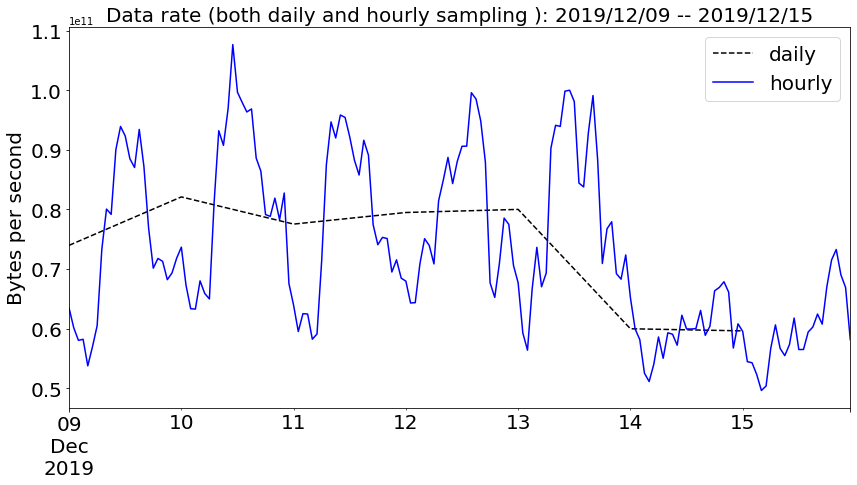
\includegraphics[width=\columnwidth]{img/BCH2_byterate.png}
          \caption{Data-rate before new year holidays}
          \label{fig:BCH2_bps}
    \end{subfigure}
    \begin{subfigure}{\linearFigSze\textwidth}
          \centering
          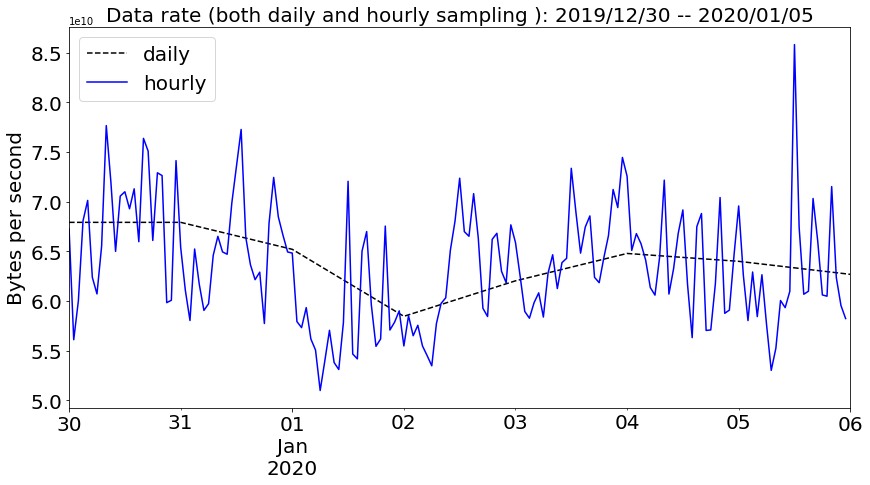
\includegraphics[width=\columnwidth]{img/CH2_byterate.png}
          \caption{Data-rate during new year holidays}
          \label{fig:CH2_bps}
    \end{subfigure}
    \caption{Impact of new year holidays on data rate}
    \label{fig:datarate_BCH_CH}
\end{figure}

\begin{figure}
    \begin{subfigure}{\linearFigSze\textwidth}
          \centering
          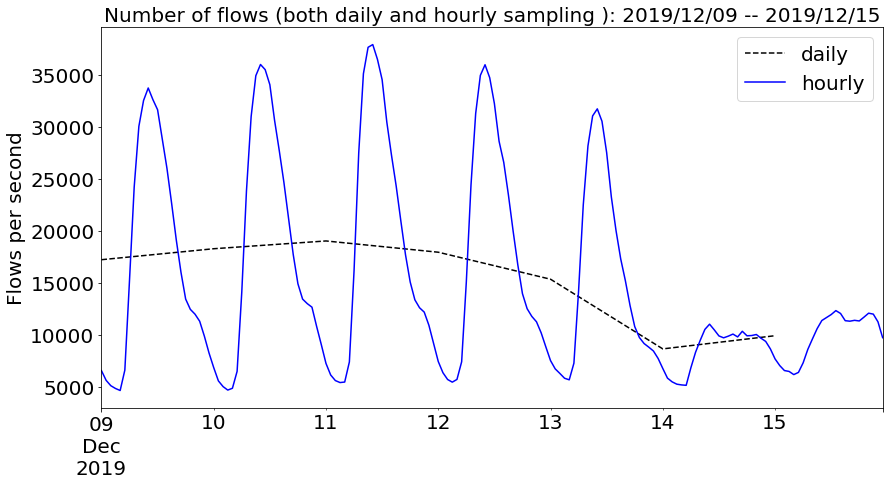
\includegraphics[width=\columnwidth]{img/BCH2_flowrate.png}
          \caption{Flow-rate before new year holidays}
          \label{fig:BCH2_fps}
    \end{subfigure}
    \begin{subfigure}{\linearFigSze\textwidth}
          \centering
          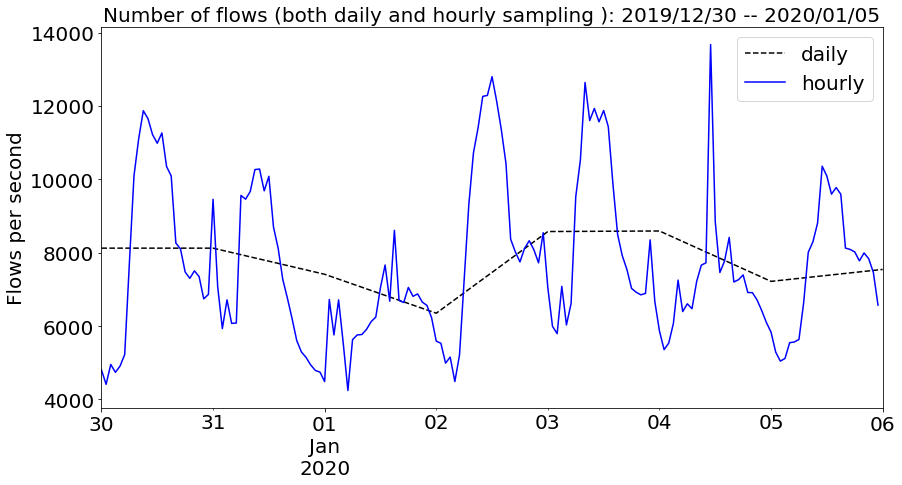
\includegraphics[width=\columnwidth]{img/CH2_flowrate.png}
          \caption{Flow-rate during new year holidays}
          \label{fig:CH2_fps}
    \end{subfigure}
    \caption{Impact of new year holidays on flow rate}
    \label{fig:flowrate_BCH_CH}
\end{figure}

\subsection{Academic and Business Traffic}
\begin{figure}
    \begin{subfigure}{\linearFigSze\textwidth}
          \centering
          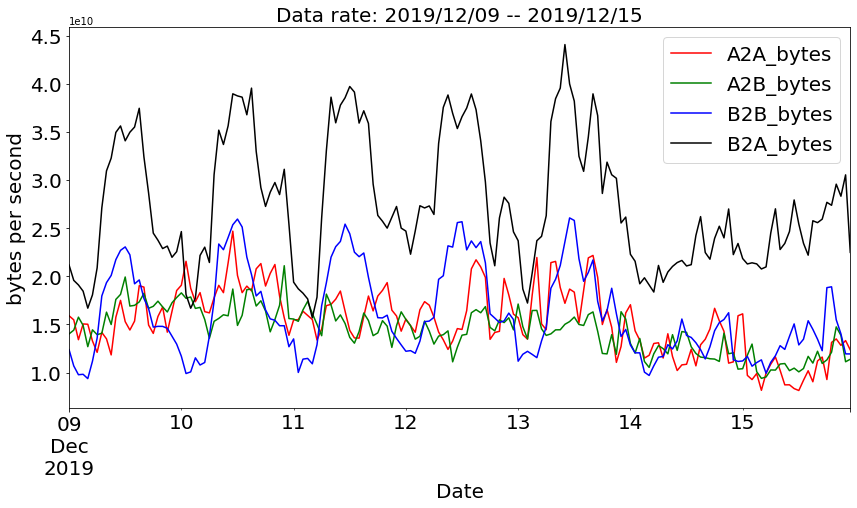
\includegraphics[width=\columnwidth]{img/BCH2_acaBus_bps.png}
          \caption{Data-rate before new year holidays}
          \label{fig:BCH2_acaBus_bps}
    \end{subfigure}
    \begin{subfigure}{\linearFigSze\textwidth}
          \centering
          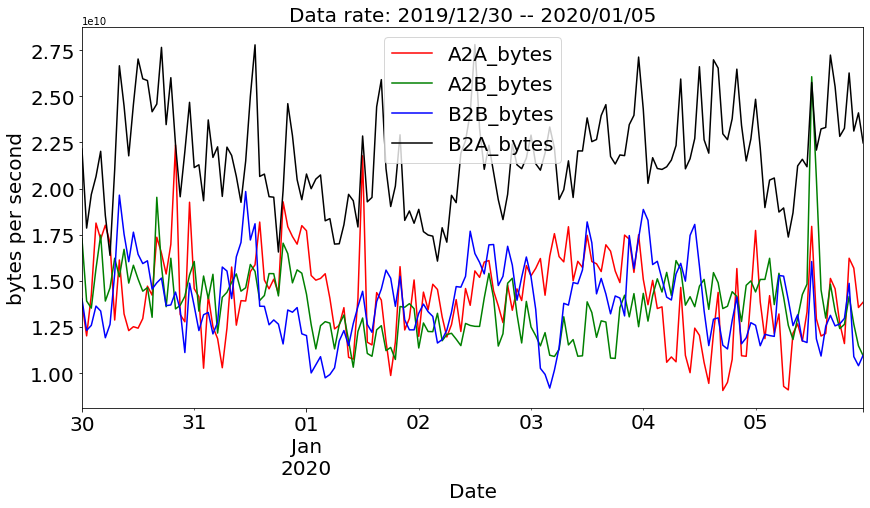
\includegraphics[width=\columnwidth]{img/CH2_acaBus_bps.png}
          \caption{Data-rate during new year holidays}
          \label{fig:CH2_acaBus_bps}
    \end{subfigure}
    \caption{Impact of new year holidays on data rate of academic and business traffic}
    \label{fig:datarate_acaBus_BCH_CH}
\end{figure}

\begin{figure}
    \begin{subfigure}{\linearFigSze\textwidth}
          \centering
          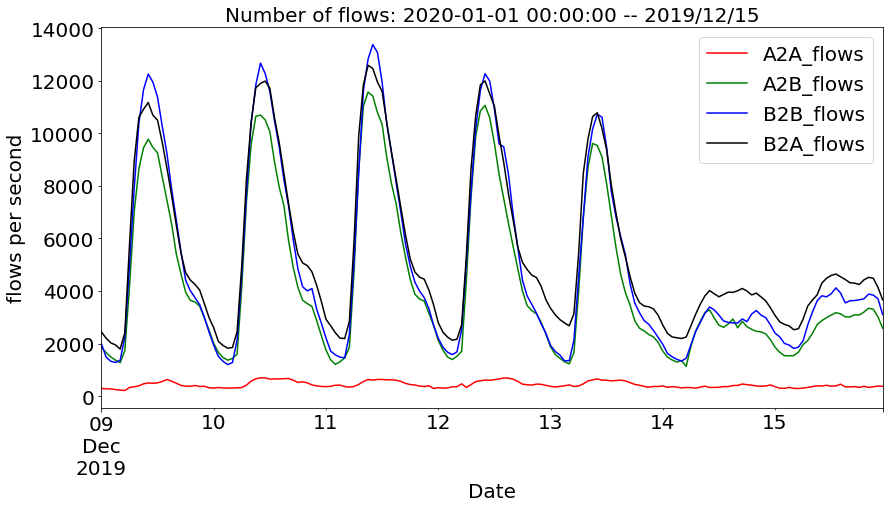
\includegraphics[width=\columnwidth]{img/BCH2_acaBus_fps.png}
          \caption{Flow-rate before new year holidays}
          \label{fig:BCH2_acaBus_fps}
    \end{subfigure}
    \begin{subfigure}{\linearFigSze\textwidth}
          \centering
          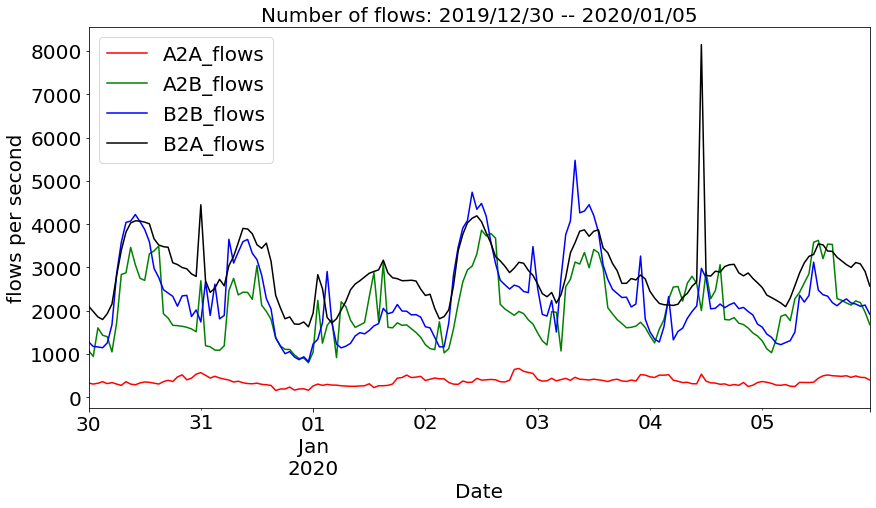
\includegraphics[width=\columnwidth]{img/CH2_acaBus_fps.png}
          \caption{Flow-rate during new year holidays}
          \label{fig:CH2_acaBus_fps}
    \end{subfigure}
    \caption{Impact of new year holidays on flow rate of academic and business traffic}
    \label{fig:flowrate_acaBus_BCH_CH}
\end{figure}

\subsection{NRENs Traffic}

\subsection{Top ASes}

\subsection{Discussion}



\section{Impact of Covid-19 on GEANT}

\subsection{Total Traffic Throughput}
Due to the COVID19 pandemic, traffic in terms of bytes dropped by almost one-third, whereas overall flows dropped by almost half. This difference in observation could be due to the nature of flows. A flow is a unidirectional sequence of packets that contains among other things an ingress interface, IP protocol, source and destination IP addresses, source and destination ports and type of service. While flows require an ingress interface and a request initiating a flow, traffic in bytes may just be machine-to-machine. This is further supported by similar trends during the Christmas/NYE holidays.

\subsection{Academic and Business Traffic}

\subsection{NRENs Traffic}

\subsection{Top ASes}

\subsection{Discussion}

\section{Comparing Covid-19 and New Year Holidays impact on GEANT}




\section{OLD}
\subsection{network Throughput}


\begin{figure*}
    \begin{subfigure}{\linearFigSze\textwidth}
          \centering
          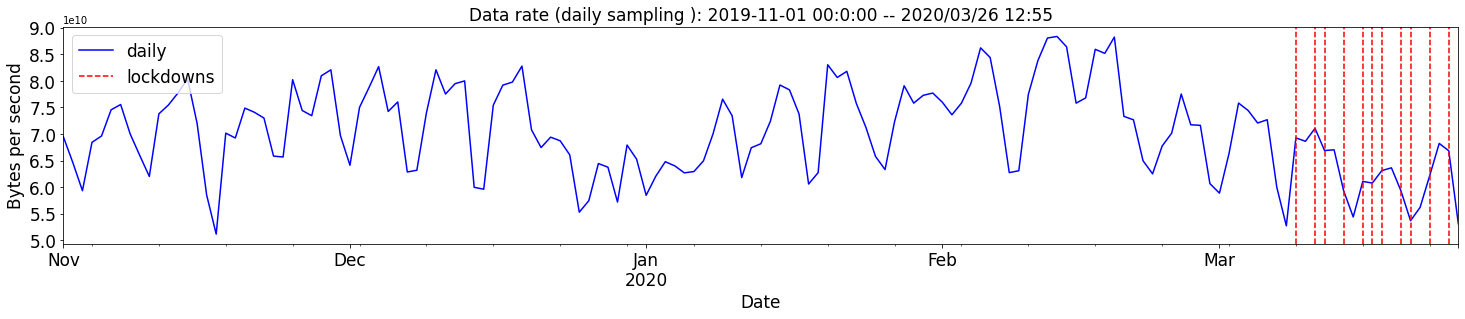
\includegraphics[width=\columnwidth]{img/traffic_trend_bps.png}
          \caption{Bytes per second}
          \label{fig:traffic_trend_bps}
    \end{subfigure}
    \begin{subfigure}{\linearFigSze\textwidth}
          \centering
          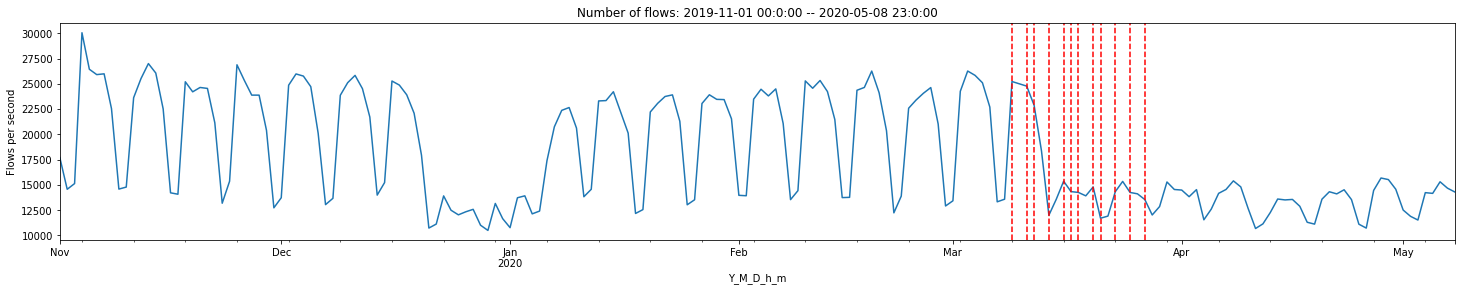
\includegraphics[width=\columnwidth]{img/traffic_trend_fps.png}
          \caption{Flow per second}
          \label{fig:traffic_trend_fps}
    \end{subfigure}
    \caption{Network Throughput}
    \label{fig:network_throughput}
\end{figure*}

The sampling of bps has faced a problem since 2020/03/26 12:55. 

\subsection{Break-down to Academic and Business}
\begin{figure*}
    \begin{subfigure}{\linearFigSze\textwidth}
          \centering
          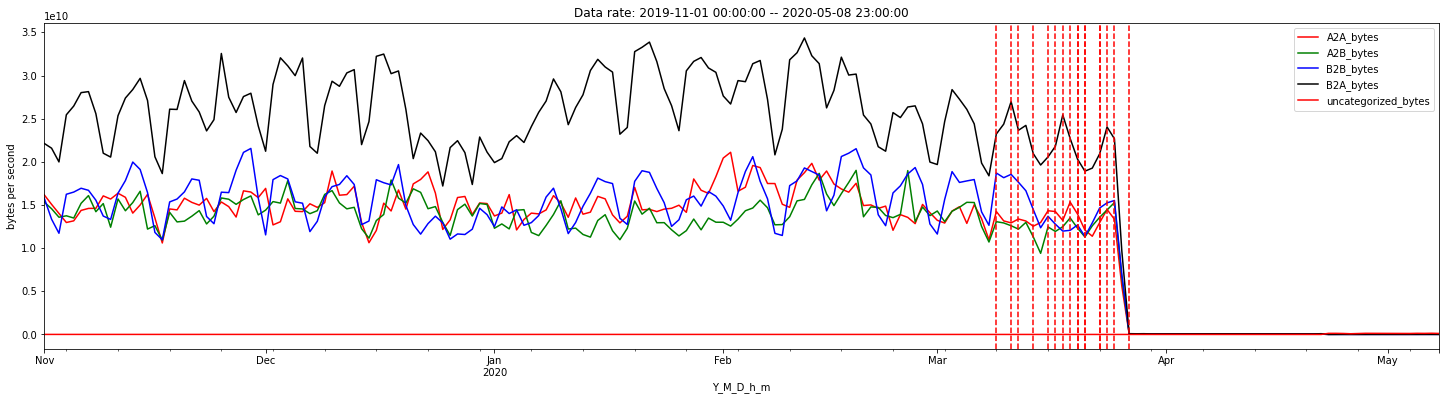
\includegraphics[width=\columnwidth]{img/traffic_trend_bps_AcaVsBus.png}
          \caption{Bytes per second}
          \label{fig:traffic_trend_acaVSbusi_bps}
    \end{subfigure}
    \begin{subfigure}{\linearFigSze\textwidth}
          \centering
          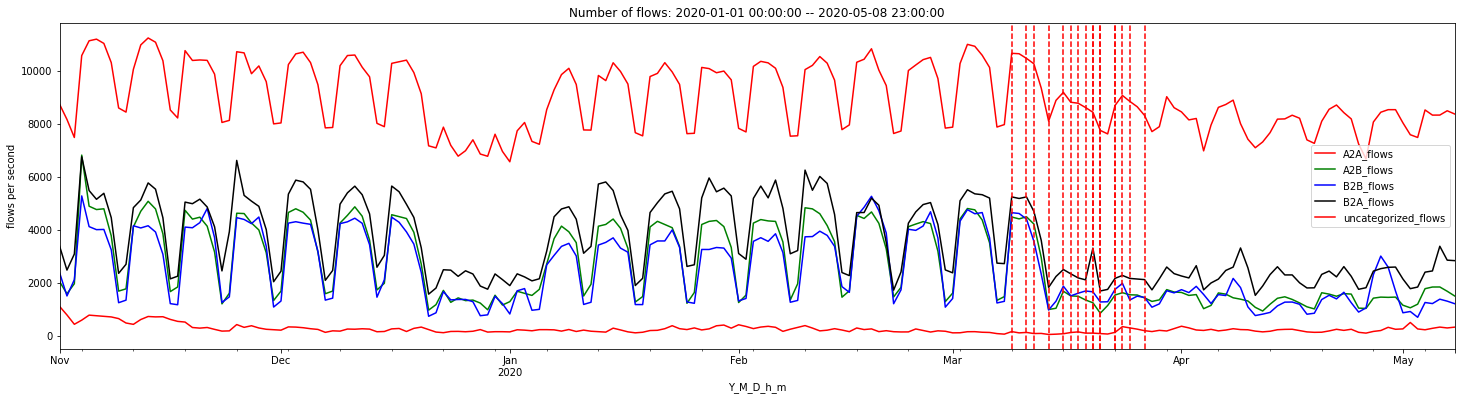
\includegraphics[width=\columnwidth]{img/traffic_trend_fps_AcaVsBus.png}
          \caption{Flow per second}
          \label{fig:traffic_trend_acaVSbusi_fps}
    \end{subfigure}
    \caption{Network Throughput Breakdown}
    \label{fig:network_throughput_breakdown}
\end{figure*}

Figure \ref{fig:nrens_bps} shows total traffic (academic and non-academic) in bytes from and to various NRENs. While it is clear that the traffic gets reduced as lockdowns start taking affect, what is more apparent is the intermittent nature of traffic spikes during the lockdown period. These traffic spikes may occur due to server routines such as updates, security patches, network monitoring, resource management and backup routines.

\section{NRENs Traffic Pattern}
\subsection{fps and bps}
\begin{figure*}
    \begin{subfigure}{\linearFigSze\textwidth}
          \centering
          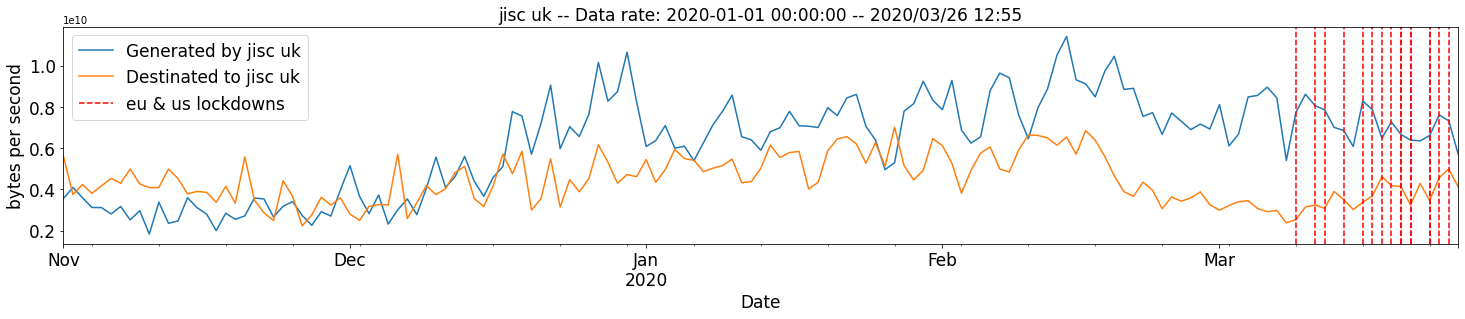
\includegraphics[width=\columnwidth]{img/jisc_bps.png}
          \caption{JISC}
          \label{fig:jisc_bps}
    \end{subfigure}
    \begin{subfigure}{\linearFigSze\textwidth}
          \centering
          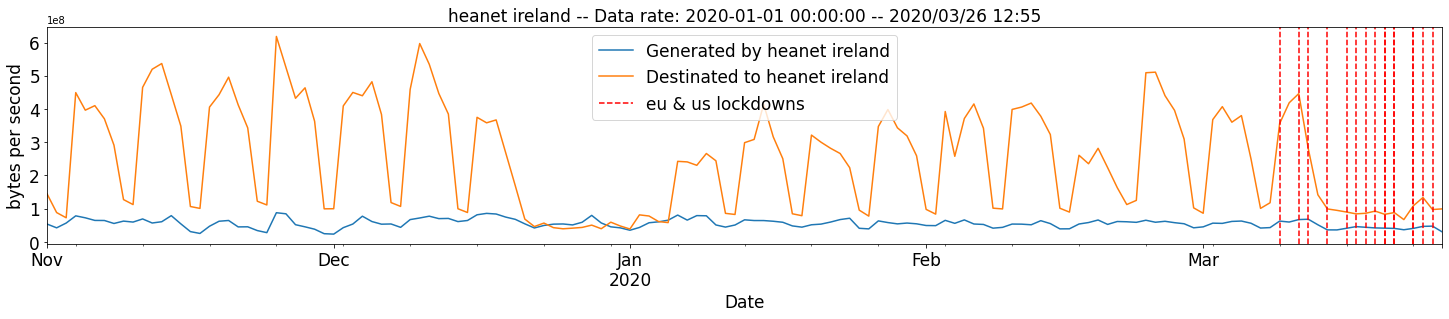
\includegraphics[width=\columnwidth]{img/heanet_bps.png}
          \caption{HEANET}
          \label{fig:HEANET_bps}
    \end{subfigure}
    \begin{subfigure}{\linearFigSze\textwidth}
          \centering
          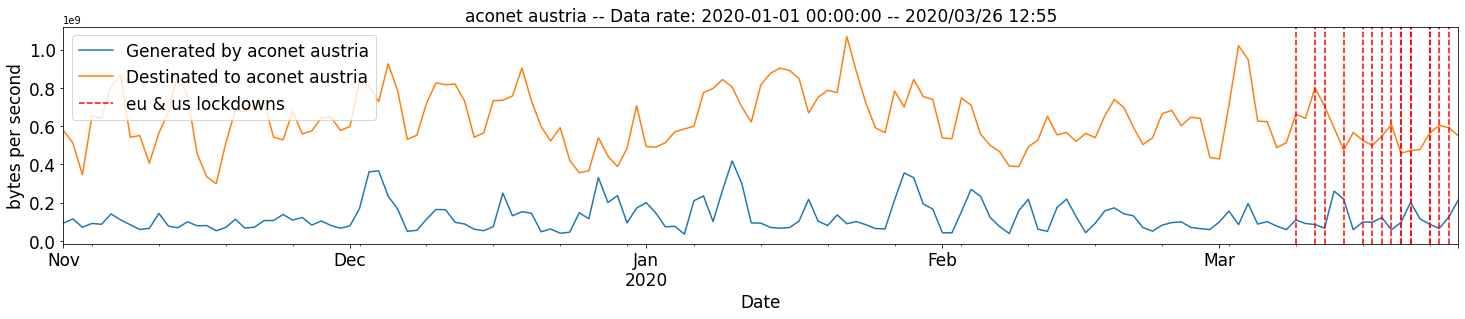
\includegraphics[width=\columnwidth]{img/aconet_bps.png}
          \caption{ACONET Austria}
          \label{fig:aconet_bps}
    \end{subfigure}
    \begin{subfigure}{\linearFigSze\textwidth}
          \centering
          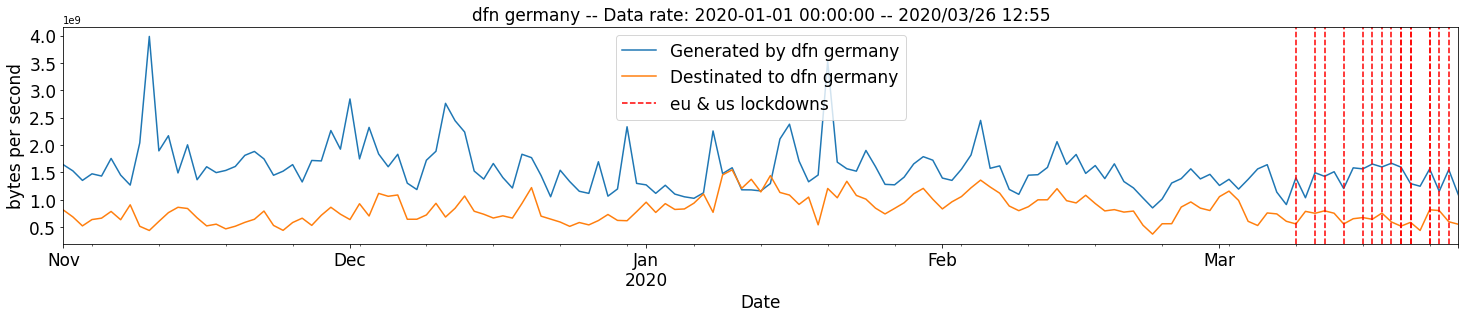
\includegraphics[width=\columnwidth]{img/dfn_bps.png}
          \caption{DFN Germany}
          \label{fig:dfn_bps}
    \end{subfigure}
    \begin{subfigure}{\linearFigSze\textwidth}
          \centering
          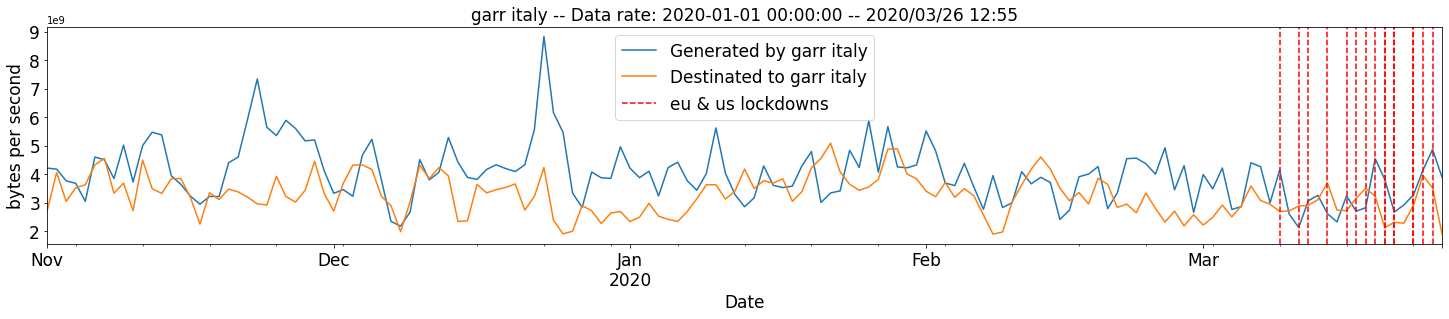
\includegraphics[width=\columnwidth]{img/garr_bps.png}
          \caption{GARR Italy}
          \label{fig:garr_bps}
    \end{subfigure}
    \begin{subfigure}{\linearFigSze\textwidth}
          \centering
          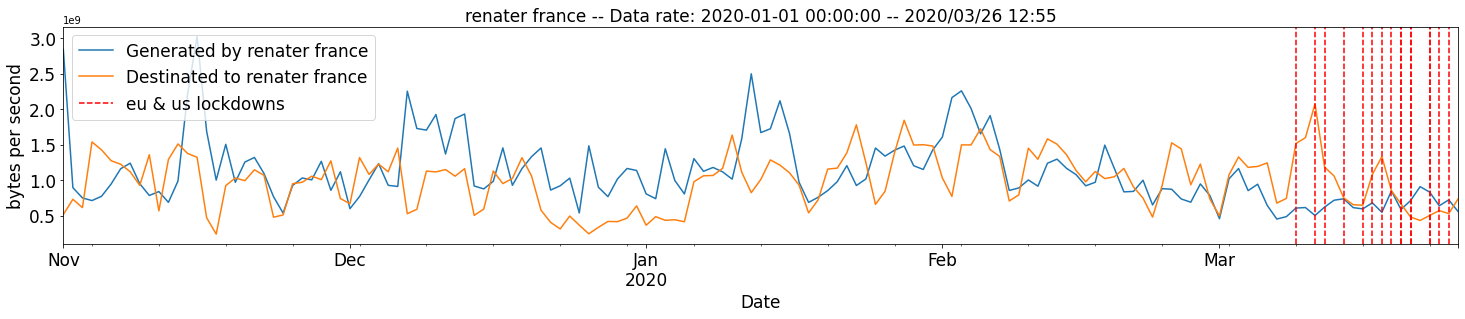
\includegraphics[width=\columnwidth]{img/rediris_bps.png}
          \caption{REDIRIS Spain}
          \label{fig:rediris_bps}
    \end{subfigure}
    \begin{subfigure}{\linearFigSze\textwidth}
          \centering
          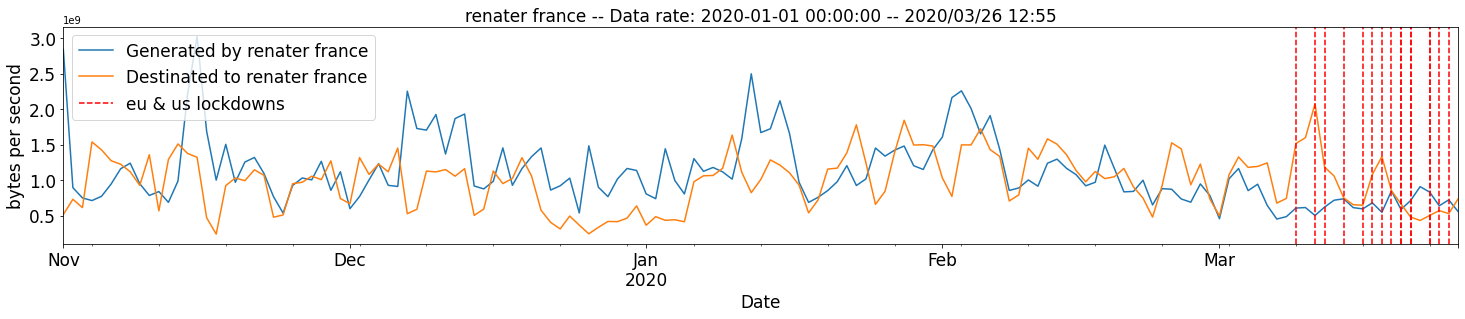
\includegraphics[width=\columnwidth]{img/renater_bps.png}
          \caption{RENATER France}
          \label{fig:renater_bps}
    \end{subfigure}
    \begin{subfigure}{\linearFigSze\textwidth}
          \centering
          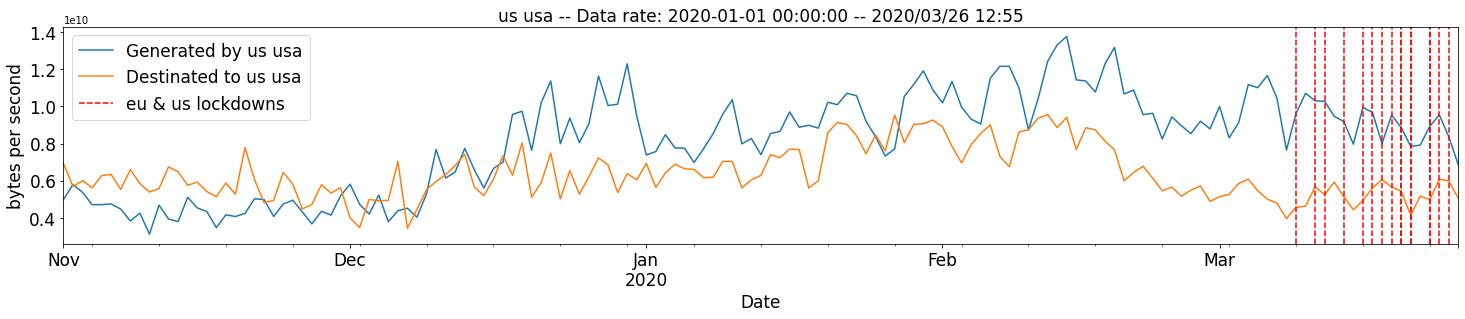
\includegraphics[width=\columnwidth]{img/us_bps.png}
          \caption{US NREN}
          \label{fig:US_bps}
    \end{subfigure}
    \begin{subfigure}{\linearFigSze\textwidth}
          \centering
          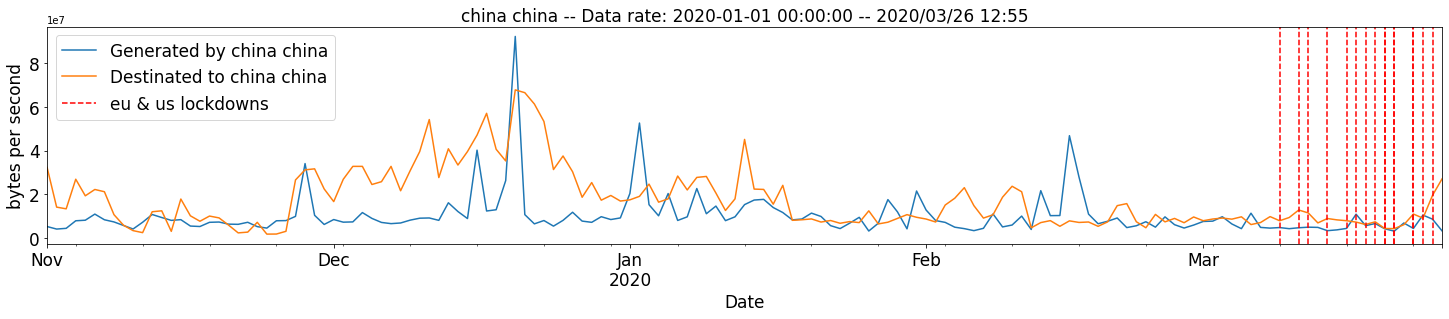
\includegraphics[width=\columnwidth]{img/china_bps.png}
          \caption{China NREN}
          \label{fig:china_bps}
    \end{subfigure}
    \caption{NRENs' Throughput (bps)}
    \label{fig:nrens_bps}
\end{figure*}

Figure \ref{fig:nrens_fps} shows trends for total traffic (academic and non-academic) in flows more clearly than traffic in bytes. Apart from JISC in the UK, DFN NREN in Germany and the NRENs in the US, all of the European NRENS show a substantial decline in flows during and after the lockdown, with some of the NRENs approaching 0 flows.

The reason for the UK, Germany and the US to deviate from the other NRENs has to do with their local handling of the pandemic and lockdown. The UK announced the lockdown but had a `soft' enforcement, Germany relied on massive test and trace campaign and the US simply did not go into the lockdown at the federal level.

\begin{figure*}
    \begin{subfigure}{\linearFigSze\textwidth}
          \centering
          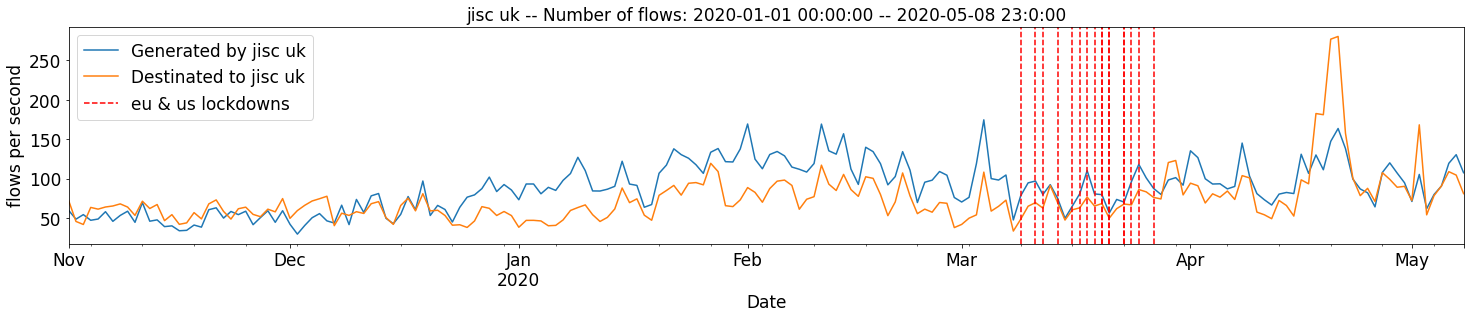
\includegraphics[width=\columnwidth]{img/jisc_fps.png}
          \caption{JISC}
          \label{fig:jisc_fps}
    \end{subfigure}
    \begin{subfigure}{\linearFigSze\textwidth}
          \centering
          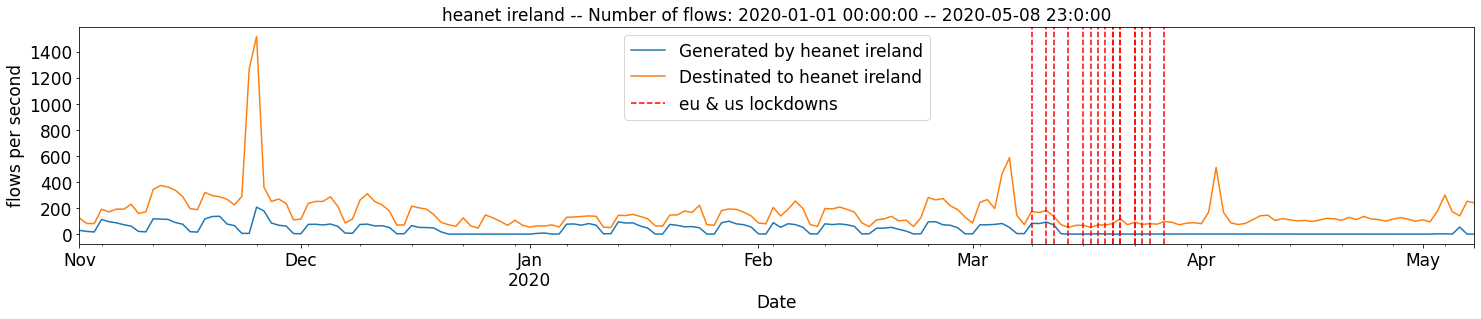
\includegraphics[width=\columnwidth]{img/heanet_fps.png}
          \caption{HEANET}
          \label{fig:HEANET_fps}
    \end{subfigure}
    \begin{subfigure}{\linearFigSze\textwidth}
          \centering
          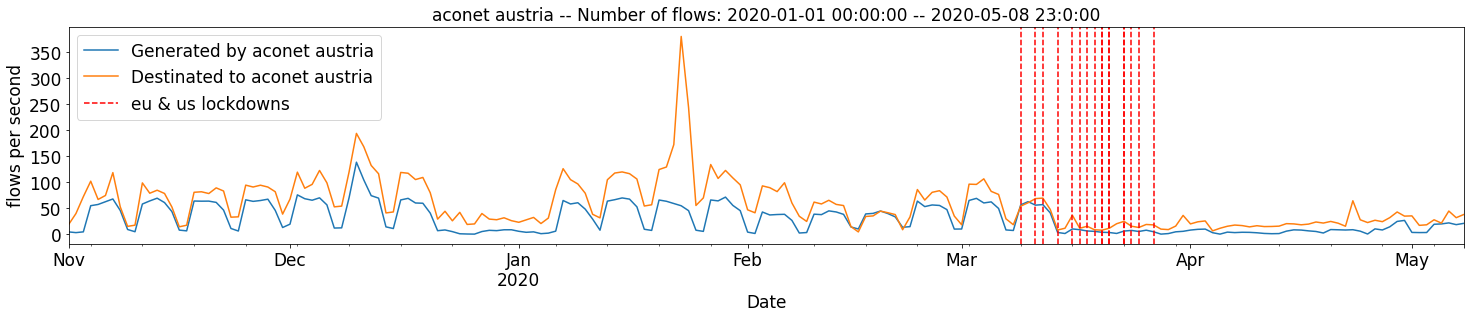
\includegraphics[width=\columnwidth]{img/aconet_fps.png}
          \caption{ACONET Austria}
          \label{fig:aconet_fps}
    \end{subfigure}
    \begin{subfigure}{\linearFigSze\textwidth}
          \centering
          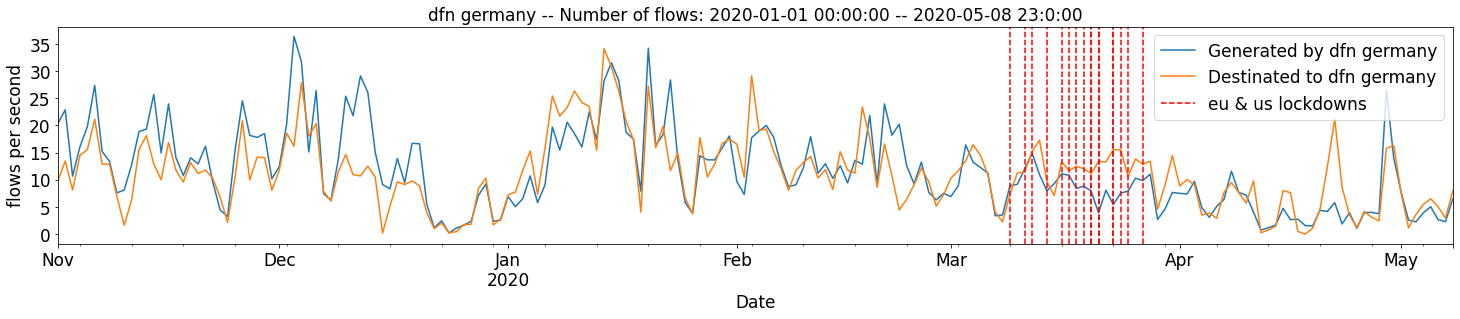
\includegraphics[width=\columnwidth]{img/dfn_fps.png}
          \caption{DFN Germany}
          \label{fig:dfn_fps}
    \end{subfigure}
    \begin{subfigure}{\linearFigSze\textwidth}
          \centering
          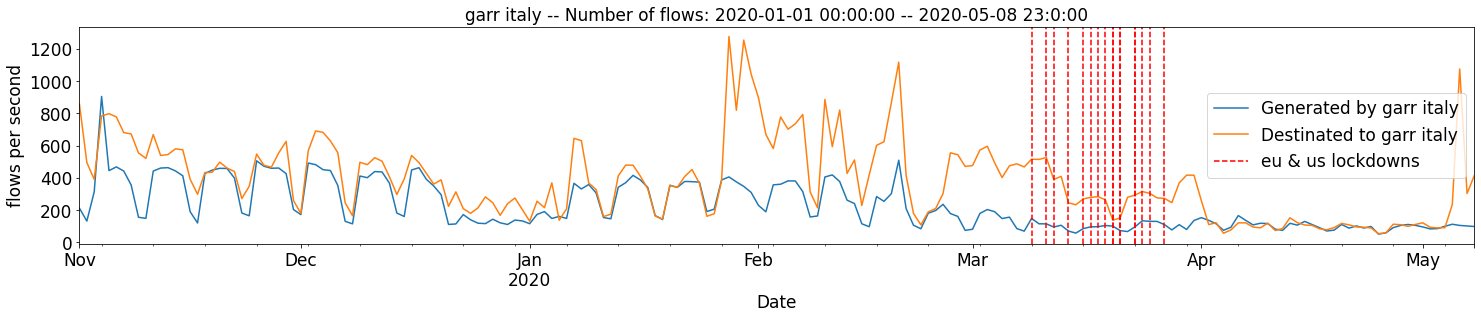
\includegraphics[width=\columnwidth]{img/garr_fps.png}
          \caption{GARR Italy}
          \label{fig:garr_fps}
    \end{subfigure}
    \begin{subfigure}{\linearFigSze\textwidth}
          \centering
          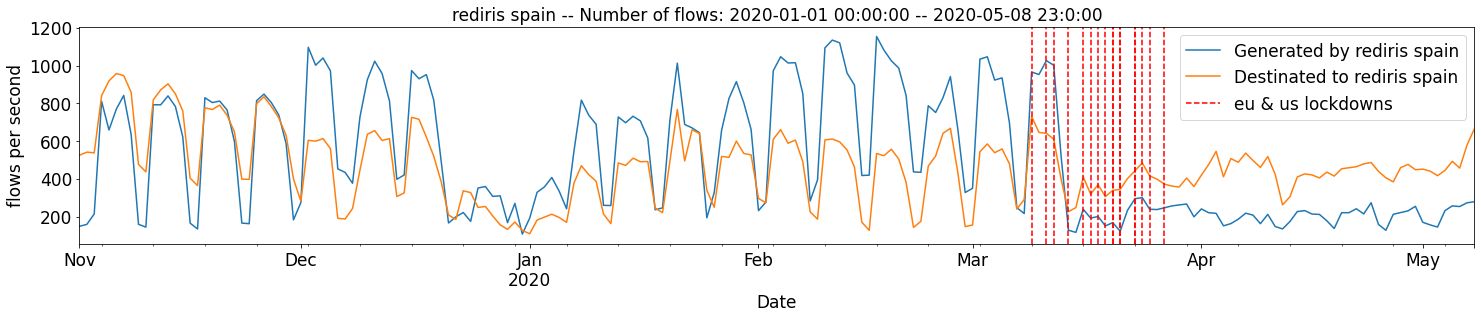
\includegraphics[width=\columnwidth]{img/rediris_fps.png}
          \caption{REDIRIS Spain}
          \label{fig:rediris_fps}
    \end{subfigure}
    \begin{subfigure}{\linearFigSze\textwidth}
          \centering
          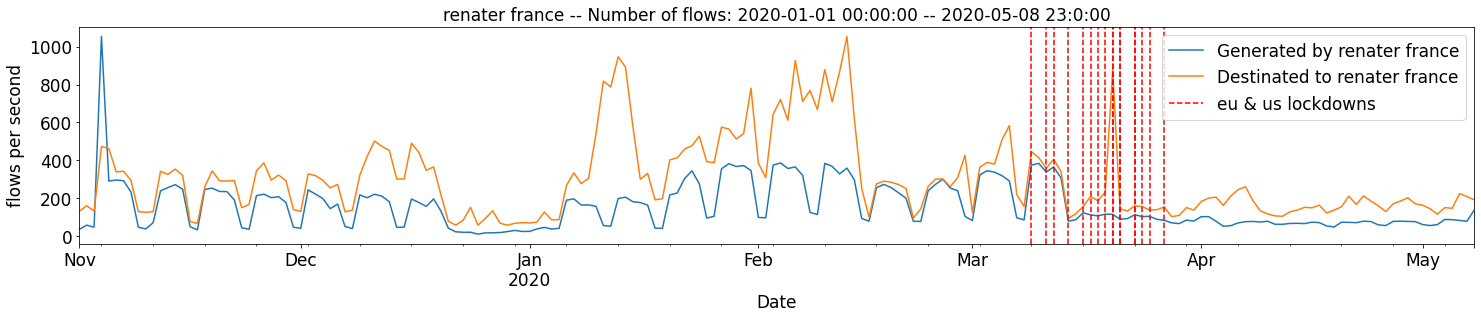
\includegraphics[width=\columnwidth]{img/renater_fps.png}
          \caption{RENATER France}
          \label{fig:renater_fps}
    \end{subfigure}
    \begin{subfigure}{\linearFigSze\textwidth}
          \centering
          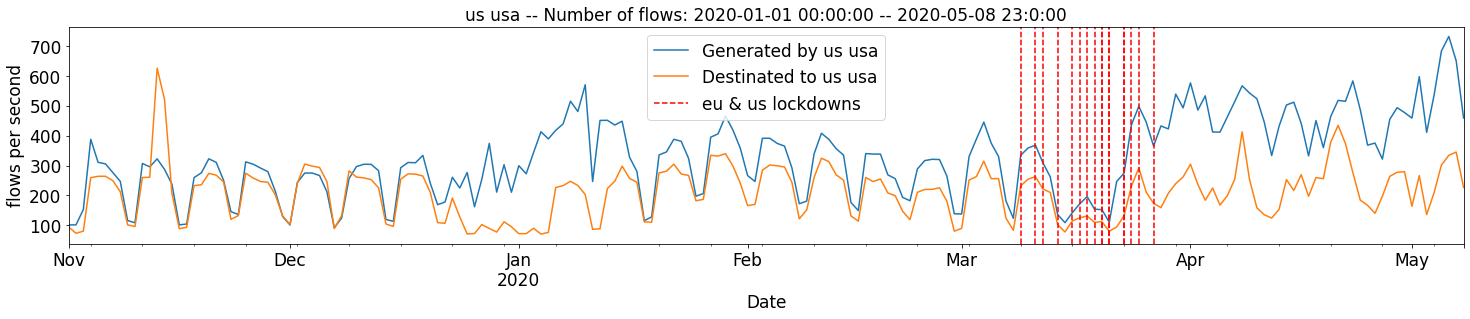
\includegraphics[width=\columnwidth]{img/us_fps.png}
          \caption{US NREN}
          \label{fig:US_fps}
    \end{subfigure}
    \begin{subfigure}{\linearFigSze\textwidth}
          \centering
          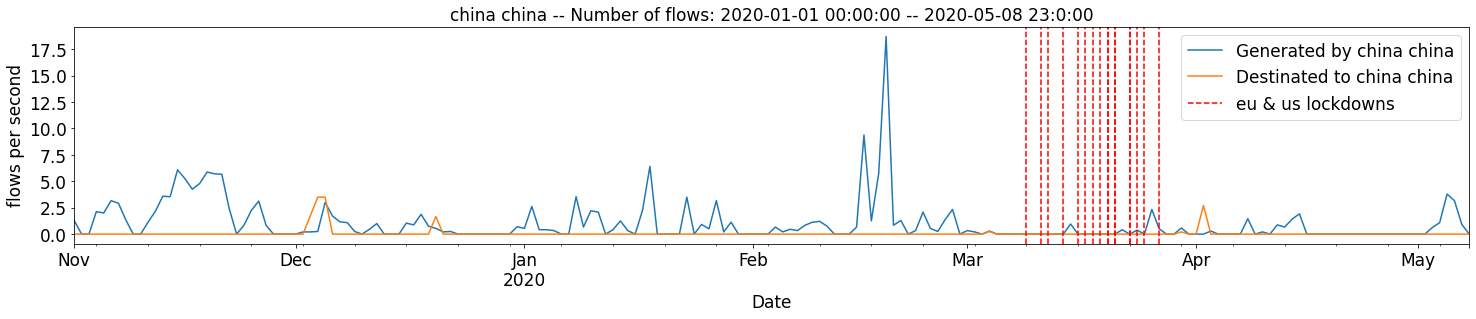
\includegraphics[width=\columnwidth]{img/china_fps.png}
          \caption{China NREN}
          \label{fig:china_fps}
    \end{subfigure}
    \caption{NRENs' Throughput (fps)}
    \label{fig:nrens_fps}
\end{figure*}

\subsection{break-down to Academic and Business}
A2A: Academic to Academic
B2B: Business to Business
Uncategorized: Small flows aggregated

The following figures show academic traffic in bytes (Figure \ref{fig:nrens_aca_bps}) and flows (Figure \ref{fig:nrens_aca_fps}) to academic ASes from observed NRENs. Though, overall academic traffic from NRENs to academic ASes shows a decline in traffic in bytes, it gives credence to the observation that machine generated NREN traffic destined to other machines of the academic ASes was still present.

\begin{figure*}
    \begin{subfigure}{\linearFigSze\textwidth}
          \centering
          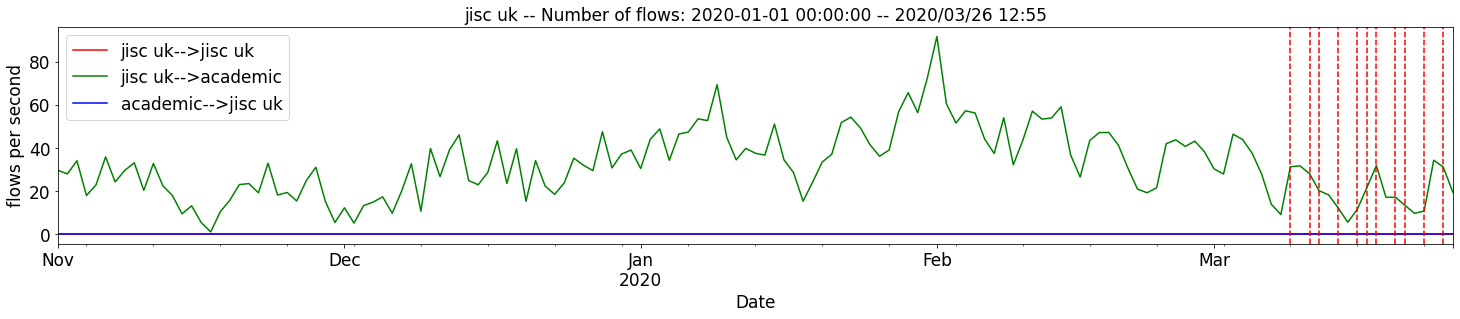
\includegraphics[width=\columnwidth]{img/jisc_aca_bps.png}
          \caption{JISC}
          \label{fig:jisc_aca_bps}
    \end{subfigure}
    % \begin{subfigure}{\linearFigSze\textwidth}
    %       \centering
    %       \includegraphics[width=\columnwidth]{img/heanet_aca_fps.png}
    %       \caption{HEANET}
    %       \label{fig:HEANET_aca_fps}
    % \end{subfigure}
    % \begin{subfigure}{\linearFigSze\textwidth}
    %       \centering
    %       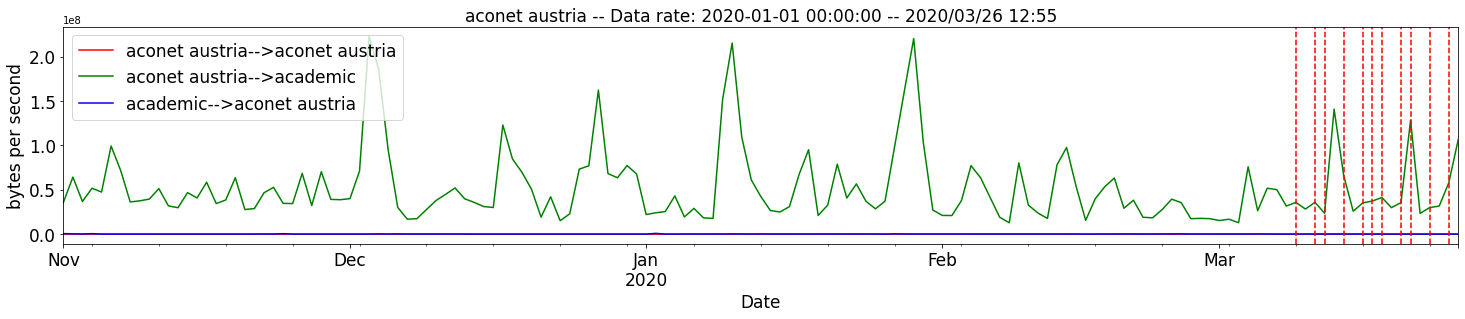
\includegraphics[width=\columnwidth]{img/aconet_aca_bps.png}
    %       \caption{ACONET Austria}
    %       \label{fig:aconet_aca_bps}
    % \end{subfigure}
    \begin{subfigure}{\linearFigSze\textwidth}
          \centering
          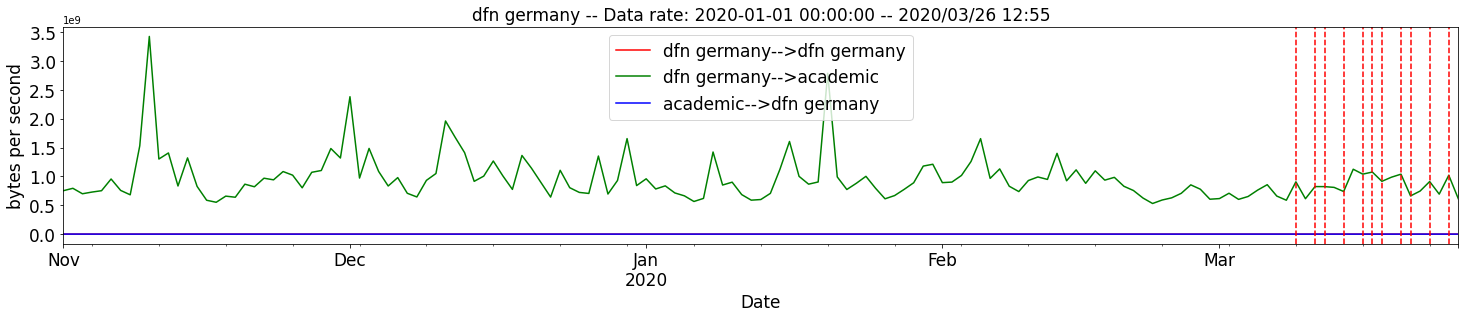
\includegraphics[width=\columnwidth]{img/dfn_aca_bps.png}
          \caption{DFN Germany}
          \label{fig:dfn_aca_bps}
    \end{subfigure}
    \begin{subfigure}{\linearFigSze\textwidth}
          \centering
          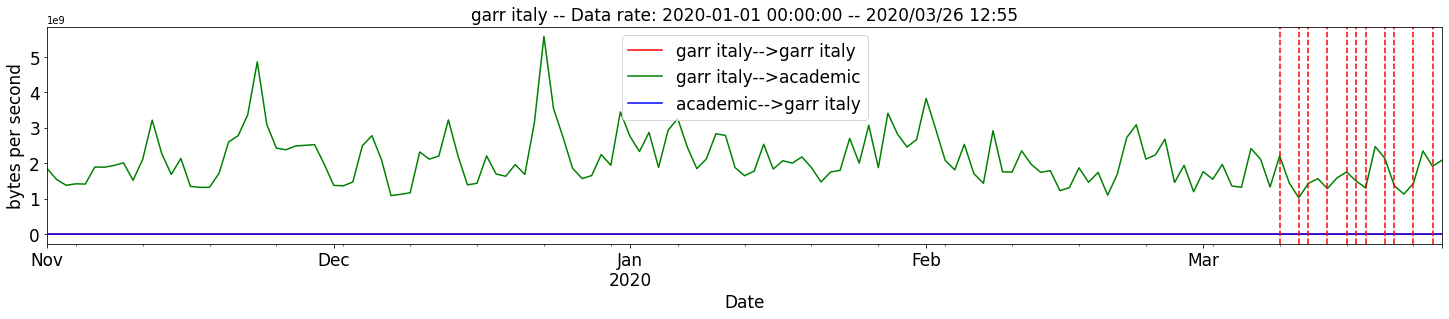
\includegraphics[width=\columnwidth]{img/garr_aca_bps.png}
          \caption{GARR Italy}
          \label{fig:garr_aca_bps}
    \end{subfigure}
    % \begin{subfigure}{\linearFigSze\textwidth}
    %       \centering
    %       \includegraphics[width=\columnwidth]{img/rediris_aca_fps.png}
    %       \caption{REDIRIS Spain}
    %       \label{fig:rediris_aca_fps}
    % \end{subfigure}
    % \begin{subfigure}{\linearFigSze\textwidth}
    %       \centering
    %       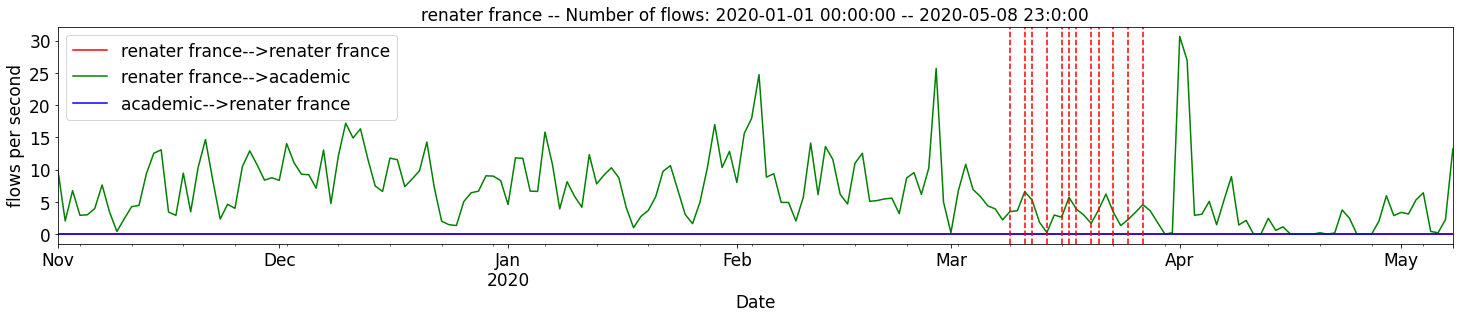
\includegraphics[width=\columnwidth]{img/renater_aca_fps.png}
    %       \caption{RENATER France}
    %       \label{fig:renater_aca_fps}
    % \end{subfigure}
    \begin{subfigure}{\linearFigSze\textwidth}
          \centering
          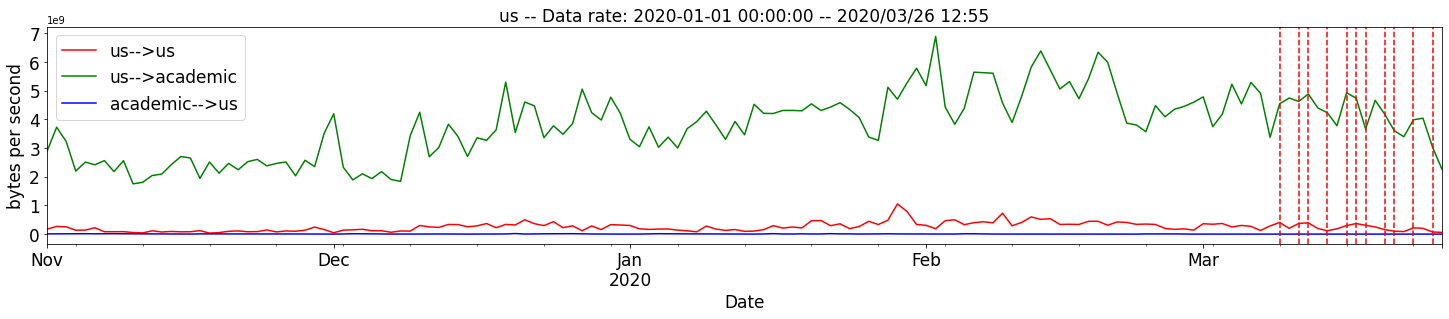
\includegraphics[width=\columnwidth]{img/us_aca_bps.png}
          \caption{US NREN}
          \label{fig:US_aca_bps}
    \end{subfigure}
    % \begin{subfigure}{\linearFigSze\textwidth}
    %       \centering
    %       \includegraphics[width=\columnwidth]{img/china_aca_fps.png}
    %       \caption{China NREN}
    %       \label{fig:china_aca_fps}
    % \end{subfigure}
    \caption{Traffic destined to Academic ASes of NRENs' (bps)}
    \label{fig:nrens_aca_bps}
\end{figure*}

That said academic traffic in flows (Figure \ref{fig:nrens_aca_fps}) to academic ASes from observed NRENs, showed a considerable decline across NRENs except the UK and the US. There is a large foreign student population in both these countries, who were left without a choice when borders closed following lockdown announcements and airlines seized serving routes. Since the students in these countries could not return to their countries of origin, they were supported by their universities and institutions to maintain residence in their student accommodation during the lockdown period, thus showing little to no change in traffic flows for JISC in the UK and in fact an increase in traffic flows in the US.

\begin{figure*}
    \begin{subfigure}{\linearFigSze\textwidth}
          \centering
          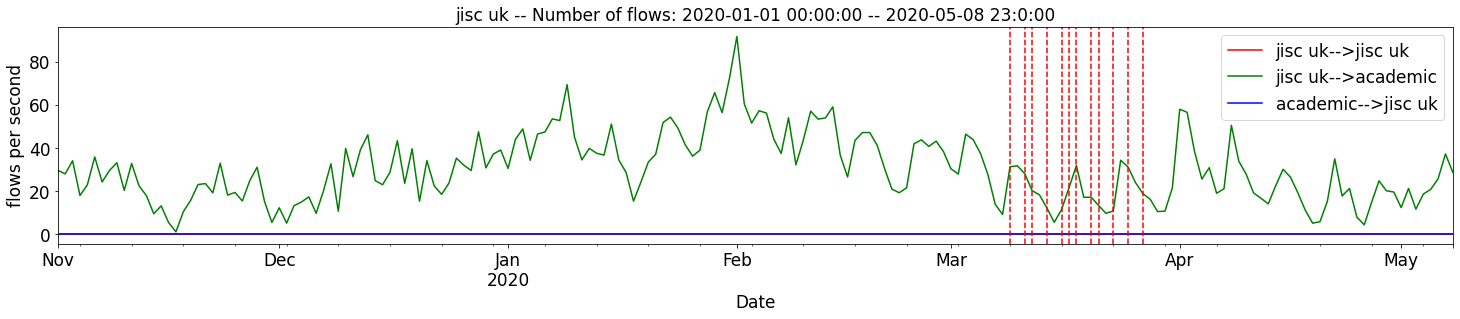
\includegraphics[width=\columnwidth]{img/jisc_aca_fps.png}
          \caption{JISC}
          \label{fig:jisc_aca_fps}
    \end{subfigure}
    % \begin{subfigure}{\linearFigSze\textwidth}
    %       \centering
    %       \includegraphics[width=\columnwidth]{img/heanet_aca_fps.png}
    %       \caption{HEANET}
    %       \label{fig:HEANET_aca_fps}
    % \end{subfigure}
    \begin{subfigure}{\linearFigSze\textwidth}
          \centering
          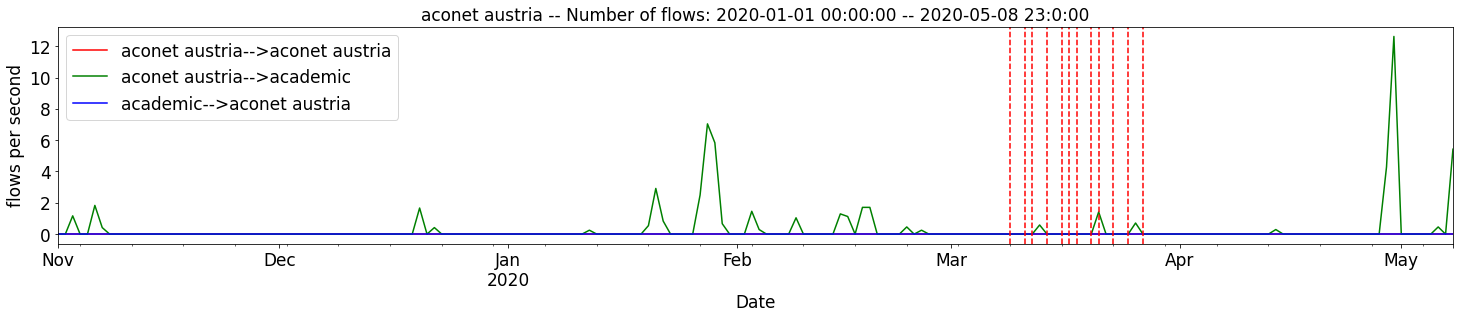
\includegraphics[width=\columnwidth]{img/aconet_aca_fps.png}
          \caption{ACONET Austria}
          \label{fig:aconet_aca_fps}
    \end{subfigure}
    \begin{subfigure}{\linearFigSze\textwidth}
          \centering
          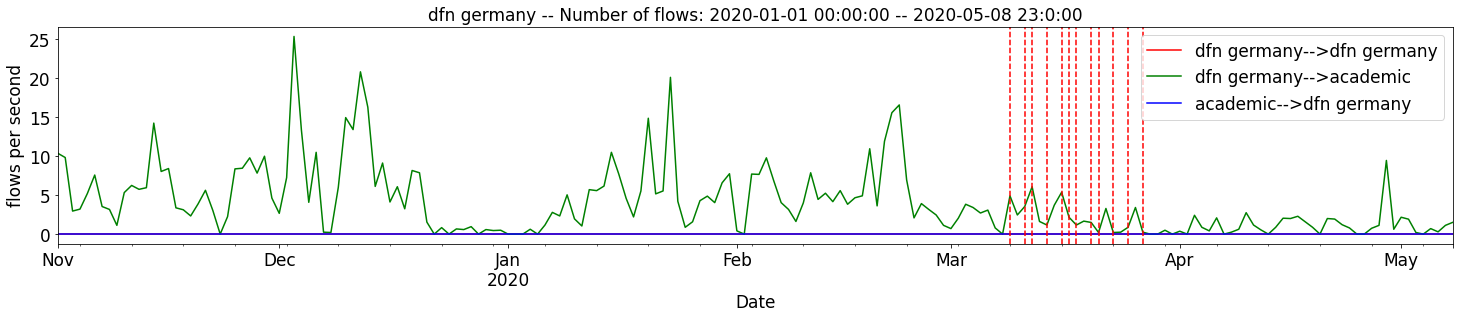
\includegraphics[width=\columnwidth]{img/dfn_aca_fps.png}
          \caption{DFN Germany}
          \label{fig:dfn_aca_fps}
    \end{subfigure}
    \begin{subfigure}{\linearFigSze\textwidth}
          \centering
          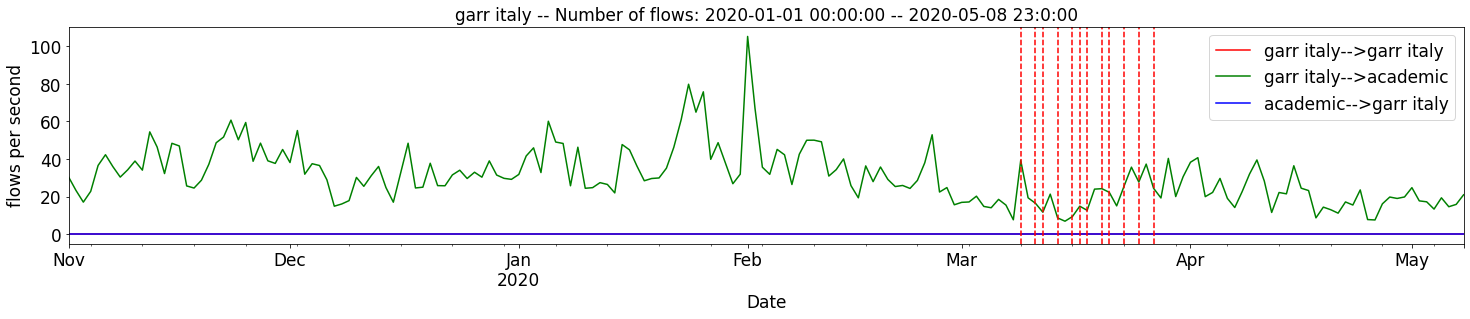
\includegraphics[width=\columnwidth]{img/garr_aca_fps.png}
          \caption{GARR Italy}
          \label{fig:garr_aca_fps}
    \end{subfigure}
    % \begin{subfigure}{\linearFigSze\textwidth}
    %       \centering
    %       \includegraphics[width=\columnwidth]{img/rediris_aca_fps.png}
    %       \caption{REDIRIS Spain}
    %       \label{fig:rediris_aca_fps}
    % \end{subfigure}
    % \begin{subfigure}{\linearFigSze\textwidth}
    %       \centering
    %       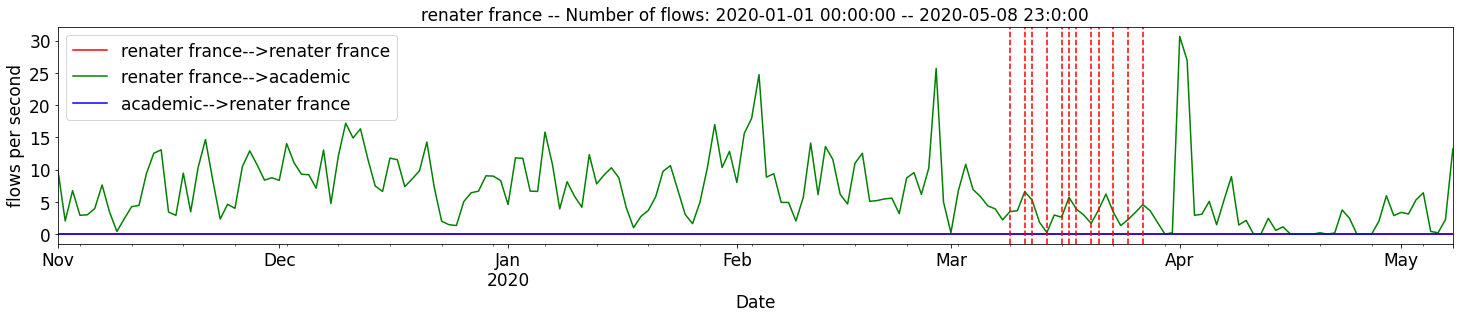
\includegraphics[width=\columnwidth]{img/renater_aca_fps.png}
    %       \caption{RENATER France}
    %       \label{fig:renater_aca_fps}
    % \end{subfigure}
    \begin{subfigure}{\linearFigSze\textwidth}
          \centering
          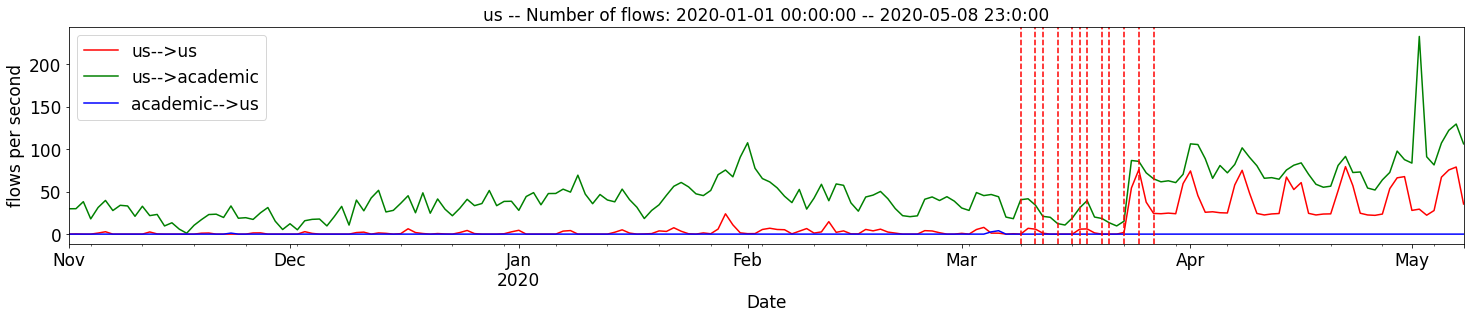
\includegraphics[width=\columnwidth]{img/us_aca_fps.png}
          \caption{US NREN}
          \label{fig:US_aca_fps}
    \end{subfigure}
    % \begin{subfigure}{\linearFigSze\textwidth}
    %       \centering
    %       \includegraphics[width=\columnwidth]{img/china_aca_fps.png}
    %       \caption{China NREN}
    %       \label{fig:china_aca_fps}
    % \end{subfigure}
    \caption{Traffic destined to Academic ASes of NRENs' (fps)}
    \label{fig:nrens_aca_fps}
\end{figure*}

Next we look at the traffic in bytes to and from non-academic networks across these NRENs. Figure \ref{fig:nrens_busi_bps} show that although there was a decline in the overall activity, the diurnal trends hold, both for non-academic incoming traffic to the NRENs as well as the outgoing to non-academic ASes. This is comparable to the period before the lockdowns and is in line with what ISPs and CDNs reported (cite sources from IMC'20 paper).

\begin{figure*}
    \begin{subfigure}{\linearFigSze\textwidth}
          \centering
          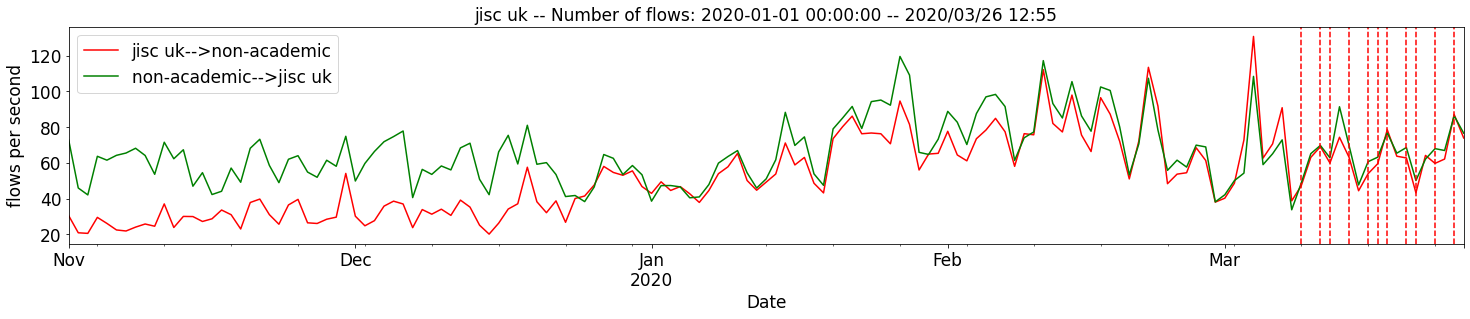
\includegraphics[width=\columnwidth]{img/jisc_busi_bps.png}
          \caption{JISC}
          \label{fig:jisc_busi_bps}
    \end{subfigure}
    % \begin{subfigure}{\linearFigSze\textwidth}
    %       \centering
    %       \includegraphics[width=\columnwidth]{img/heanet_busi_fps.png}
    %       \caption{HEANET}
    %       \label{fig:HEANET_busi_fps}
    % \end{subfigure}
    % \begin{subfigure}{\linearFigSze\textwidth}
    %       \centering
    %       \includegraphics[width=\columnwidth]{img/aconet_busi_bps.png}
    %       \caption{ACONET Austria}
    %       \label{fig:aconet_aca_bps}
    % \end{subfigure}
    \begin{subfigure}{\linearFigSze\textwidth}
          \centering
          \includegraphics[width=\columnwidth]{img/dfn_busi_bps.png}
          \caption{DFN Germany}
          \label{fig:dfn_busi_bps}
    \end{subfigure}
    \begin{subfigure}{\linearFigSze\textwidth}
          \centering
          \includegraphics[width=\columnwidth]{img/garr_busi_bps.png}
          \caption{GARR Italy}
          \label{fig:garr_busi_bps}
    \end{subfigure}
    % \begin{subfigure}{\linearFigSze\textwidth}
    %       \centering
    %       \includegraphics[width=\columnwidth]{img/rediris_busi_fps.png}
    %       \caption{REDIRIS Spain}
    %       \label{fig:rediris_aca_fps}
    % \end{subfigure}
    % \begin{subfigure}{\linearFigSze\textwidth}
    %       \centering
    %       \includegraphics[width=\columnwidth]{img/renater_busi_fps.png}
    %       \caption{RENATER France}
    %       \label{fig:renater_aca_fps}
    % \end{subfigure}
    \begin{subfigure}{\linearFigSze\textwidth}
          \centering
          \includegraphics[width=\columnwidth]{img/us_busi_bps.png}
          \caption{US NREN}
          \label{fig:US_busi_bps}
    \end{subfigure}
    % \begin{subfigure}{\linearFigSze\textwidth}
    %       \centering
    %       \includegraphics[width=\columnwidth]{img/china_busi_fps.png}
    %       \caption{China NREN}
    %       \label{fig:china_aca_fps}
    % \end{subfigure}
    \caption{Traffic to and from non-Academic ASes of NRENs' (bps)}
    \label{fig:nrens_busi_bps}
\end{figure*}

The trends for non-academic traffic in flows (Figure \ref{fig:nrens_busi_fps}) shows apparent differences from the behaviour observed in Figure \ref{fig:nrens_busi_bps}. The UK shows high incoming traffic from non-academic ASes that follows no regular pattern and shows spikes in demand following the lockdown. The US shows an initial dip during the lockdown period and then shows an increase but no regular pattern. In fact, the traffic to and from the non-academic ASes in the US showed at par behaviour before the lockdown period, but distinctly more traffic from the NRENs to non-academic ASes since the lockdown. Germany showed no real signs of change except the volume and Austrian NRENs showed a decline since and following the lockdown period.

\begin{figure*}
    \begin{subfigure}{\linearFigSze\textwidth}
          \centering
          \includegraphics[width=\columnwidth]{img/jisc_busi_fps.png}
          \caption{JISC}
          \label{fig:jisc_busi_fps}
    \end{subfigure}
    % \begin{subfigure}{\linearFigSze\textwidth}
    %       \centering
    %       \includegraphics[width=\columnwidth]{img/heanet_busia_fps.png}
    %       \caption{HEANET}
    %       \label{fig:HEANET_busi_fps}
    % \end{subfigure}
    \begin{subfigure}{\linearFigSze\textwidth}
          \centering
          \includegraphics[width=\columnwidth]{img/aconet_busi_fps.png}
          \caption{ACONET Austria}
          \label{fig:aconet_busi_fps}
    \end{subfigure}
    \begin{subfigure}{\linearFigSze\textwidth}
          \centering
          \includegraphics[width=\columnwidth]{img/dfn_busi_fps.png}
          \caption{DFN Germany}
          \label{fig:dfn_busi_fps}
    \end{subfigure}
    % \begin{subfigure}{\linearFigSze\textwidth}
    %       \centering
    %       \includegraphics[width=\columnwidth]{img/garr_busi_fps.png}
    %       \caption{GARR Italy}
    %       \label{fig:garr_busi_fps}
    % \end{subfigure}
    % \begin{subfigure}{\linearFigSze\textwidth}
    %       \centering
    %       \includegraphics[width=\columnwidth]{img/rediris_busi_fps.png}
    %       \caption{REDIRIS Spain}
    %       \label{fig:rediris_aca_fps}
    % \end{subfigure}
    % \begin{subfigure}{\linearFigSze\textwidth}
    %       \centering
    %       \includegraphics[width=\columnwidth]{img/renater_busi_fps.png}
    %       \caption{RENATER France}
    %       \label{fig:renater_aca_fps}
    % \end{subfigure}
    \begin{subfigure}{\linearFigSze\textwidth}
          \centering
          \includegraphics[width=\columnwidth]{img/us_busi_fps.png}
          \caption{US NREN}
          \label{fig:US_busi_fps}
    \end{subfigure}
    % \begin{subfigure}{\linearFigSze\textwidth}
    %       \centering
    %       \includegraphics[width=\columnwidth]{img/china_busi_fps.png}
    %       \caption{China NREN}
    %       \label{fig:china_aca_fps}
    % \end{subfigure}
    \caption{Traffic to and from non-Academic ASes of NRENs' (fps)}
    \label{fig:nrens_busi_fps}
\end{figure*}

\subsection{histogram}

\begin{figure*}
    \begin{subfigure}{\histFigSze\textwidth}
          \centering
          \includegraphics[width=\columnwidth]{img/jisc_hist_fps.png}
          \caption{JISC}
          \label{fig:jisc_hist_fps}
    \end{subfigure}
    % \begin{subfigure}{\linearFigSze\textwidth}
    %       \centering
    %       \includegraphics[width=\columnwidth]{img/heanet_hist_fps.png}
    %       \caption{HEANET}
    %       \label{fig:HEANET_busi_fps}
    % \end{subfigure}
    \begin{subfigure}{\histFigSze\textwidth}
          \centering
          \includegraphics[width=\columnwidth]{img/aconet_hist_fps.png}
          \caption{ACONET Austria}
          \label{fig:aconet_hist_fps}
    \end{subfigure}
    \begin{subfigure}{\histFigSze\textwidth}
          \centering
          \includegraphics[width=\columnwidth]{img/dfn_hist_fps.png}
          \caption{DFN Germany}
          \label{fig:dfn_hist_fps}
    \end{subfigure}
    \begin{subfigure}{\histFigSze\textwidth}
          \centering
          \includegraphics[width=\columnwidth]{img/garr_hist_fps.png}
          \caption{GARR Italy}
          \label{fig:garr_hist_fps}
    \end{subfigure}
    \begin{subfigure}{\histFigSze\textwidth}
          \centering
          \includegraphics[width=\columnwidth]{img/rediris_hist_fps.png}
          \caption{REDIRIS Spain}
          \label{fig:rediris_hist_fps}
    \end{subfigure}
    \begin{subfigure}{\histFigSze\textwidth}
          \centering
          \includegraphics[width=\columnwidth]{img/renater_hist_fps.png}
          \caption{RENATER France}
          \label{fig:renater_hist_fps}
    \end{subfigure}
    \begin{subfigure}{\histFigSze\textwidth}
          \centering
          \includegraphics[width=\columnwidth]{img/us_hist_fps.png}
          \caption{US NREN}
          \label{fig:US_hist_fps}
    \end{subfigure}
    % \begin{subfigure}{\histFigSze\textwidth}
    %       \centering
    %       \includegraphics[width=\columnwidth]{img/china_hist_fps.png}
    %       \caption{China NREN}
    %       \label{fig:china_aca_fps}
    % \end{subfigure}
    \caption{Flow per Second Histogram}
    \label{fig:nrens_hist_fps}
\end{figure*}

\subsection{Sankey Plot}
In these plots, the top-n one-way communications are considered. For example, consider

A->B: 10 bps (meaning that there is a traffic flow of 10 bps from A to B)
A->C: 1 bps
A->D: 9bps
B->C:11bps
B->D: 3bps
B->A:5bps
then the top-3 one-way communications are:
A->B:10bps
A-D:9bps
B-C:11bps

AS-Level Analysis: every AS is considered as a unique entity. Each NREN has one or more AS-number. Each of these numbers are considered as one unique entity.

NREN-Level Analysis: all ASes belonging to an NREN are aggregated together, e.g., consider AS7 is in customer cone of AS786 (JISC). The traffic generated by AS7 and destinated to AS-x (AS7 -> AS-x) will be considered as AS786 -> AS-x. Besides, if there are more than one ASN assigned to an NREN, these ASNes would be aggregated into one, e.g., if AS786 and AS133084 are both assigned to JISC then we replace AS133084 with AS786 everywhere.

\begin{figure*}
    \begin{subfigure}{\boxFigSze\textwidth}
          \centering
          \includegraphics[width=\columnwidth]{img/sankey_20200318_NRENlevel_bps.png}
          \caption{20200318}
          \label{fig:top_generating_fps}
    \end{subfigure}\\
    \begin{subfigure}{\boxFigSze\textwidth}
          \centering
          \includegraphics[width=\columnwidth]{img/sankey_20200319_NRENlevel_bps.png}
          \caption{20200319}
          \label{fig:top_receiving_bps}
    \end{subfigure}
    \caption{bps}
    \label{fig:sankey_bps}
\end{figure*}

\begin{figure*}
    \begin{subfigure}{\boxFigSze\textwidth}
          \centering
          \includegraphics[width=\columnwidth]{img/sankey_20200318_NRENlevel_fps.png}
          \caption{20200318}
          \label{fig:top_generating_fps}
    \end{subfigure}\\
    \begin{subfigure}{\boxFigSze\textwidth}
          \centering
          \includegraphics[width=\columnwidth]{img/sankey_20200319_NRENlevel_fps.png}
          \caption{20200319}
          \label{fig:top_receiving_fps}
    \end{subfigure}
    \caption{fps}
    \label{fig:sankey_bps}
\end{figure*}

\section{ASes}

\red{For top ASes we will need to know the overlap (i.e. common ASes) for measurement criteria. That is, how many top ASes in terms of generating traffic measured in bps are in the top ASes list if measured in terms of fps. And vice versa, e.g. receiving traffic in bps and fps, etc.}

\subsection{Top ASes fps and bps (box plot)}
In the following, top ASes are specified. The approach used to specify the top ASes is 'top over time': average the total output of each AS during the sampling period, and select the top x ASes.
Each AS may generate traffic or receives traffic, therefore, plots are divided into two categories 'Top ASes Generating Traffic' and 'Top ASes Receiving Traffic'.
\begin{figure*}
    \begin{subfigure}{\boxFigSze\textwidth}
          \centering
          \includegraphics[width=\columnwidth]{img/top_AS_generating_bps.png}
          \caption{Generating Traffic}
          \label{fig:top_generating_bps}
    \end{subfigure}
    \begin{subfigure}{\boxFigSze\textwidth}
          \centering
          \includegraphics[width=\columnwidth]{img/top_AS_receiving_bps.png}
          \caption{Receiving Traffic}
          \label{fig:top_receiving_bps}
    \end{subfigure}
    \caption{Top ASes (bps)}
    \label{fig:top_AS_bps}
\end{figure*}
\begin{figure*}
    \begin{subfigure}{\boxFigSze\textwidth}
          \centering
          \includegraphics[width=\columnwidth]{img/top_AS_generating_fps.png}
          \caption{Generating Traffic}
          \label{fig:top_generating_fps}
    \end{subfigure}\\
    \begin{subfigure}{\boxFigSze\textwidth}
          \centering
          \includegraphics[width=\columnwidth]{img/top_AS_receiving_fps.png}
          \caption{Receiving Traffic}
          \label{fig:top_receiving_fps}
    \end{subfigure}
    \caption{Top ASes (fps)}
    \label{fig:top_AS_fps}
\end{figure*}

\end{document}
